%%%%%%%%%%%%%%%%%%%%%%%%%%%%%%%%%%%%%%%%%
% Masters/Doctoral Thesis 
% LaTeX Template
% Version 2.3 (25/3/16)
%
% This template has been downloaded from:
% http://www.LaTeXTemplates.com
%
% Version 2.x major modifications by:
% Vel (vel@latextemplates.com)
%
% This template is based on a template by:
% Steve Gunn (http://users.ecs.soton.ac.uk/srg/softwaretools/document/templates/)
% Sunil Patel (http://www.sunilpatel.co.uk/thesis-template/)
%
% Template license:
% CC BY-NC-SA 3.0 (http://creativecommons.org/licenses/by-nc-sa/3.0/)
%
%%%%%%%%%%%%%%%%%%%%%%%%%%%%%%%%%%%%%%%%%

%-------------------------------------------------------------------------------
%	PACKAGES AND OTHER DOCUMENT CONFIGURATIONS
%-------------------------------------------------------------------------------

\documentclass[
11pt,
spanish,
singlespacing,
parskip,
headsepline,
]{MastersDoctoralThesis}

\usepackage{tikz}
\usetikzlibrary{positioning,shapes,arrows,automata,fit,calc,babel}

\usepackage[utf8]{inputenc}
\usepackage[T1]{fontenc}

\usepackage{palatino}

\usepackage[backend=bibtex,natbib=true, style=numeric, sorting=none]{biblatex}

\addbibresource{references.bib}

\usepackage[autostyle=true]{csquotes}

\usepackage{caption}
\usepackage{subcaption}

%------------------------
\usepackage{listings}
\urlstyle{same}
\hyphenation{biblatex}
%--------------------------

\usepackage{color}

%-------------------------------------------------------------------------------
%	MARGIN SETTINGS
%-------------------------------------------------------------------------------

\geometry{
	paper=a4paper,
	inner=2cm,
	outer=3.3cm,
	bindingoffset=2cm,
	top=1.5cm,
	bottom=1.5cm,
}

%-------------------------------------------------------------------------------
%	INFORMACIÓN DE LA MEMORIA
%-------------------------------------------------------------------------------

\thesistitle{Monitoreo ambiental integrado a Enterprise Buildings Integrator de Honeywell} % \ttitle
\degree{Especialista en Internet de las Cosas} % \degreename
\author{Ing. Gonzalo Nahuel Vaca} % \authorname
\supervisor{Esp. Ing. Pablo Almada (FIUBA-UTN)} % \supname
\juradoUNO{Christian Yanez Flores (pertenencia)} % \jur1name
\juradoDOS{Lucas Fabricio Monzón Languasco (pertenencia)} % \jur2name
\juradoTRES{Daniel Marquez (pertenencia)} % \jur3name
\fechaINICIO{mayo de 2020}
\fechaFINAL{abril de 2021}

\subject{Memoria del Trabajo Final de la Carrera de Especialización en Internet de las Cosas de la UBA} % \subjectname
\keywords{Sistemas Embebidos, CESE, FIUBA} % \keywordnames
\university{Universidad de Buenos Aires} % \univname
\faculty{{Facultad de Ingeniería}} % \facname
\department{Departamento de Electrónica} % \deptname
\group{{Laboratorio de Sistemas Embebidos}} % \groupname


\hypersetup{pdftitle=\ttitle}
\hypersetup{pdfauthor=\authorname}
\hypersetup{pdfkeywords=\keywordnames}


\newcaptionname{spanish}{\acknowledgementname}{Agradecimientos}
\newcaptionname{spanish}{\authorshipname}{Declaración de Autoría}
\newcaptionname{spanish}{\abbrevname}{Glosario}
\newcaptionname{spanish}{\byname}{por}

\renewcommand{\lstlistingname}{Algoritmo}
\renewcommand{\lstlistlistingname}{Índice de \lstlistingname s}

\renewcommand{\listtablename}{Índice de Tablas}
\renewcommand{\tablename}{Tabla} 

\addtolength{\footnotesep}{2mm}

\begin{document}

\frontmatter

\pagestyle{plain}

%-------------------------------------------------------------------------------
%	CARÁTULA
%-------------------------------------------------------------------------------

\begin{titlepage}
\begin{center}



\includegraphics[width=.8\textwidth]{./Figures/logoFIUBA.png}
\vspace{2cm}

\textsc{\huge{Carrera de Especialización en\\ \vspace{5px} Internet de las Cosas}}
\vspace{.5cm}

\textsc{\Large Memoria del Trabajo Final}\\[1cm]

{\huge \bfseries \ttitle\par}\vspace{0.4cm}

\vfill

\vspace{2cm}
\LARGE\textbf{Autor:\\
\authorname}\\

\vspace{1.5cm}

\large
{Director:} \\
{\supname}
 
\vspace{1cm}
Jurados:\\	
\jurunoname\\
\jurdosname\\
\jurtresname

\vspace{2cm}

\textit{Este trabajo fue realizado en las Ciudad Autónoma de Buenos Aires,\\ entre \fechaINICIOname \hspace{1px} y \fechaFINALname.}
\end{center}
\end{titlepage}


%-------------------------------------------------------------------------------
%	RESUMEN - ABSTRACT 
%-------------------------------------------------------------------------------

\begin{abstract}
\addchaptertocentry{\abstractname}

\centering

Esta memoria describe la implementación de una solución realizada para los laboratorios Gador, en donde se adapta su sistema de automatización de edificios y gestión empresarial marca Honeywell con una red de sensores inalámbricos que utilizan un protocolo de comunicación que este sistema no puede interpretar.

Se logró cumplir con las necesidades de Gador utilizando contenidos vistos en las asignaturas de este pos-grado. Se creó una arquitectura de datos, se implementaron protocolos de comunicaciones, se programaron servidores web y se implementó un sistema de despliegue automático y orquestación de la aplicación.

\end{abstract}

%-------------------------------------------------------------------------------
%	LISTA DE CONTENIDOS/FIGURAS/TABLAS
%-------------------------------------------------------------------------------
\renewcommand{\listtablename}{Índice de Tablas}

\tableofcontents

\listoffigures

\listoftables

%-------------------------------------------------------------------------------
%	CONTENIDO DE LA MEMORIA  - DEDICATORIA
%-------------------------------------------------------------------------------

\dedicatory{\textbf{Dedicado a la memoria del Ing. Valeriy Omelchenko}}

%-------------------------------------------------------------------------------
%	CONTENIDO DE LA MEMORIA  - CAPÍTULOS
%-------------------------------------------------------------------------------

\mainmatter

\pagestyle{thesis}

\renewcommand{\tablename}{Tabla} 

\chapter{Introducción General}

\label{Chapter1} % \ref{Chapter1} 
\label{IntroGeneral}

%-------------------------------------------------------------------------------

\newcommand{\keyword}[1]{\textbf{#1}}
\newcommand{\tabhead}[1]{\textbf{#1}}
\newcommand{\code}[1]{\texttt{#1}}
\newcommand{\file}[1]{\texttt{\bfseries#1}}
\newcommand{\option}[1]{\texttt{\itshape#1}}
\newcommand{\grados}{$^{\circ}$}

%-------------------------------------------------------------------------------

El capítulo presenta las necesidades a satisfacer y una introducción técnica. El objetivo es proveer de conceptos básicos para comprender el resto de la memoria.

\section{Motivación}
\label{motivacion}

	\subsection{Necesidades generales}
	
		Se analiza la situación de la industria local, que despertó el interés de realizar el proyecto.

		\subsubsection{Progreso tecnológico}

			La producción de bienes y servicios experimentó una serie de cambios, que reemplazaron distintos talentos humanos. Se identifican cuatro etapas, denominadas \emph{revoluciones industriales}.
		
			La primera consistió en sustituir las fuerzas físicas de hombres y bestias, en favor de nuevas fuentes de energía para obtener trabajo. Como el vapor o la electricidad. 

			La segunda revolución industrial suplantó la capacidad de polivalencia al crear líneas de montaje, fue el inicio de la organización productiva moderna.

			Un tercer hito fue la llegada de la electrónica y robótica, se reemplazó la motricidad fina y gruesa, y control manual de actuadores. 

			La etapa actual (\emph{industria 4.0}) consiste en superar algunas capacidades cognitivas, al interconectar dispositivos y ordenadores. Logrando persistencia en las mediciones, y su análisis usando inteligencia artificial.
	
		\subsubsection{Modernización}

			Las empresas locales están retrasadas en su progreso tecnológico, muchas no incorporaron sistemas electrónicos en sus procesos o productos. Es necesario crear un sistema que logre adaptar la tecnología en uso.

		\subsubsection{Comercio internacional}
			
			El avance tecnológico modifica el marco normativo de las naciones, para cumplir con los nuevos requerimientos jurídicos, se necesita tener un mínimo de capital. El retraso tecnológico ya no solo genera una pérdida de competitividad, sino que también impide que las empresas coloquen sus mercancías en otros países. Por incumplimiento en normas de calidad productiva, o de protección del medio ambiente.

	\subsection{Necesidades del cliente}
		
		\subsubsection{Gador S.A}
		
			\emph{Gador S.A} es una compañía cuya misión es \emph{producir medicamentos para la salud humana, con la mejor calidad disponible, y ponerlos al alcance de la comunidad a precios accesibles}. La empresa decidió ser el cliente del proyecto realizado.
			
			\emph{Gador} tiene la necesidad de medir las condiciones ambientales de sus depósitos y cuartos productivos. En esos lugares se dispusieron sensores de temperatura y humedad, las mediciones son recogidas por \emph{Controladores Lógicos Programables (PLC)}, los \emph{PLC} luego reenvían los datos a un servidor \emph{Enterprise Buildings Integrator (EBI)} que fue comprado con una licencia \emph{Modbus universal} y permite comunicarse con los dispositivos en campo utilizando solo ese protocolo. Las conexiones entre las partes se encuentra visualizada en la figura \ref{fig:redGador}.
			
			El principal problema de la arquitectura descripta es que el protocolo \emph{Modbus} fue diseñado en el año 1979 y no es apto para integrarse a las tecnologías de la cuarta revolución industrial. Se necesita un sistema que lo adapte.
			
			\begin{figure}[h]
				\centering
				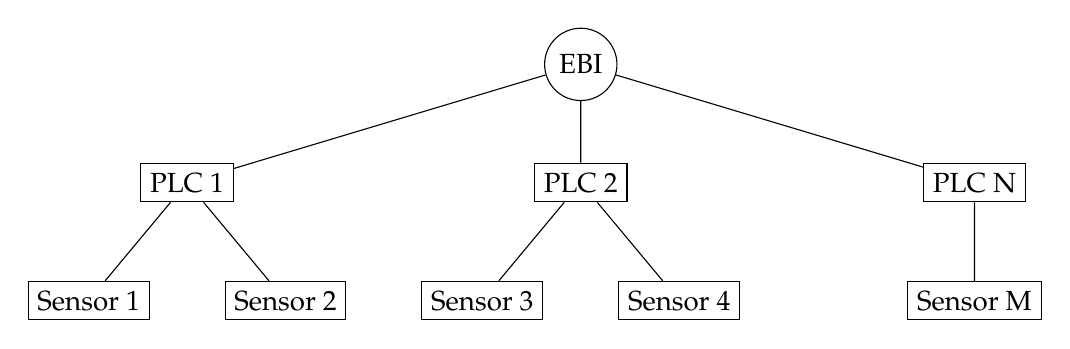
\begin{tikzpicture}[level 1/.style={sibling distance=5cm},
									level 2/.style={sibling distance=2.5cm}]
					\node[circle,draw]{EBI}
						child{
							node[rectangle,draw]{PLC 1}
								child[rectangle,draw]{node[rectangle,draw]{Sensor 1}}
								child[rectangle,draw]{node[rectangle,draw]{Sensor 2}}
							}
						child{
							node[rectangle,draw]{PLC 2}
								child{node[rectangle,draw]{Sensor 3}}
								child{node[rectangle,draw]{Sensor 4}}
							}
						child{
							node[rectangle,draw]{PLC N}
								child{node[rectangle,draw]{Sensor M}}
							}
					;
				\end{tikzpicture}
				\caption{Red industrial Gador.}
				\label{fig:redGador}
			\end{figure}
		
		\subsubsection{Marco normativo}
		
			Para acceder al mercado estadounidense, se deben satisfacer los requerimientos del \emph{Code of Federal Regulations - Title 21 - Food and Drugs Chapter - Part 11 (21CFR11)}. Esta es la principal razón para utilizar el sistema \emph{EBI}, ya que el producto se encuentra aprobado por la \emph{FDA}, por lo tanto, es indispensable que continúe operando aún cuando los protocolos que utiliza son antiguos. Tampoco es económicamente viable reemplazarlo por un producto moderno que esté aprobado por la \emph{FDA}, se debe ingresar a la industria 4.0 sin incurrir en grandes erogaciones.

		\subsubsection{Metrología}
		
			La metrología es el estudio de las mediciones. En el caso de \emph{Gador}, los datos de temperatura solo son válidos si los dispositivos se someten a un plan de calibración y a una reubicación periódica según estudios de mapeo térmico. Los estudios obtienen los puntos críticos del volumen del ambiente, que son las posiciones a ocupar por los instrumentos.
			
			Las recurrentes migraciones de sensores provocan costosos procesos de certificación de cableados, para evitarlos se requiere un protocolo de comunicación inalámbrica que sea compatible con la cuarta revolución industrial.
			
			La incorrecta gestión de dispositivos impacta negativamente en el funcionamiento de \emph{EBI}. La tarea no puede lograrse usando \emph{PLCs}, se necesitan puntos de agregación y sensores de mayor complejidad.

\section{Introducción técnica}
\label{introTecnica}

	Para facilitar la comprensión de las tecnologías involucradas, se presentan categorizadas en un modelo de \emph{Capas estandarizadas de IoT}. En él se separan los conocimientos según su función, identificando cinco especies. Percepción, red, procesamiento, aplicación y negocio. Como se detalla en la tabla \ref{tab:modeloCapas}.
	
	\begin{table}
		\centering
		\begin{tabular}{c|cccc}
			Capa 			& 				& 			& 			& 			\\ \hline
			Negocio 		& Logs 			& Usuarios 	& 			& 			\\
			Aplicación 		& Docker 		& Backend 	& Frontend	& Servicios	\\
			Procesamiento 	& MongoDB 		& 			& 			& 			\\
			Red 			& Modbus 		& MQTT 		& Websocker & HTTP 		\\
			Percepción 		& Temperatura 	& Humedad 	& 			& 			\\
		\end{tabular}
		\caption{\label{tab:modeloCapas}Modelo de capas IoT}
	\end{table}
	
	\subsection{Capa de percepción}
	\label{capaPercepcion}
	
		La capa está conformada por los sensores inalámbricos que miden temperatura y humedad.
		
		\subsubsection{Temperatura}
		
			La temperatura es la excitación mecánica (vibraciones) de los átomos que componen la materia. Para medirla existen métodos electrónicos y mecánicos. Los mecánicos se basan en la expansión y contracción de los materiales al experimentar cambios térmicos, un ejemplo son los termómetros de columna de mercurio.
		
			La temperatura puede ser medida de forma electrónica, sus variaciones producen cambios en la resistencia que los materiales presentan al paso de la corriente eléctrica. Algunas sustancias (conductores y aislantes) cuando incrementan su temperatura, aumentan su oposición, al crecer su radio atómico y por lo tanto generar un número mayor de colisiones de las partículas que forman la corriente eléctrica (electrones). Otros materiales (semiconductores) disminuyen su oposición al liberar electrones de valencia y facilitar de esta manera la circulación de corriente.
		
			Otra manera de medir temperatura usando propiedades electrónicas, es unir dos metales para formar un termopar, las diferencias térmicas producen una pequeña fuente de tensión eléctrica. Se puede visualizar como una batería que produce corriente gracias a la temperatura.
		
		\subsubsection{Humedad}
		
			La humedad se refiere a la capacidad del aire para transportar partículas de agua. Si la humedad es alta, significa que se está llegando al punto donde el aire ya no puede absorber más agua, a medida que la humedad baja el aire se aleja del punto de saturación. La cantidad de agua que el aire puede sostener depende de la presión atmosférica y de la temperatura.
		
			Una manera de medir la humedad sin involucrar electrónica es utilizando un psicrómetro, que está formado por dos termómetros, uno seco y otro con bulbo húmedo. Se utiliza una tabla donde se especifica cuál es la humedad relativa del aire en función de las diferencias de temperatura.
		
			Las mediciones electrónicas de humedad se basan en la modificación de las propiedades dialéctricas de los materiales, esto es que tanto se alinean los electrones al someter la sustancia a un campo eléctrico. Como resultado se altera el campo eléctrico original. La medición del campo es función de la humedad del aire.
		
	\subsection{Capa de red}
	\label{capaRed}
	
		Esta capa agrupa las tecnologías que permiten la conectividad de los dispositivos y ordenadores.
	
		\subsubsection{HTTP}
		
			El protocolo \emph{HTTP} permite realizar una petición de datos y recursos siguiendo una arquitectura de cliente/servidor. El cliente inicia la sesión y realiza un pedido, el servidor responde al pedido y se cierra la comunicación. Existe la variante \emph{HTTPS} que agrega seguridad en la comunicación.
		
		\subsubsection{WebSocket}
		
			Este protocolo es una mejora respecto de \emph{HTTP}, proporciona un canal de comunicación bidireccional donde el cliente y el servidor pueden enviarse mensajes de forma espontánea. Permite realizar \emph{streaming} de contenido o aplicaciones de mensajería como un \emph{chat}.
		
		\subsubsection{Modbus}
		
			\emph{Modbus} es un protocolo basado en el esquema de cliente/servidor diseñado para dispositivos industriales sometidos a las limitaciones tecnológicas del año 1979. En consecuencia, su diseño no es adecuado para la \emph{industria 4.0}
		
		\subsubsection{MQTT}
		
			\emph{MQTT} se basa en un modelo de publicación/subscripción, donde algunos dispositivos se subscriben a un \emph{topic} y otros dispositivos realizan publicaciones. Quienes están subscritos escuchan las publicaciones. El protocolo está diseñado para funcionar en dispositivos que necesitan un código ligero que no consuma un gran ancho de banda. El estándar es compatible con las actuales tecnologías y es una mejora respecto de \emph{Modbus}. En la figura \ref{fig:mqttEjemplo}, se observa como un sensor publica una medición al \emph{broker} y este lo reparte entre los clientes 1 y 3 que se encuentran subscritos, sin embargo el cliente 2 es ignorado ya que no se encuentra en el mismo \emph{topic}.
						
			\begin{figure}[h]
				\centering
				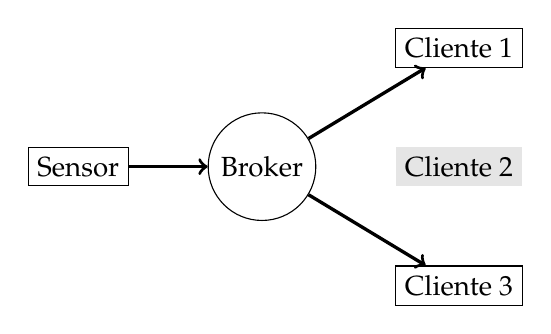
\begin{tikzpicture}
					
					\tikzstyle{broker} = [circle,draw=black]
					\tikzstyle{publish} = [rectangle,draw=black]
					\tikzstyle{subscribe} = [rectangle,draw=black]
					\tikzstyle{notsuscribe} = [rectangle,fill=black!10]
					\tikzstyle{flecha} = [->,very thick]
				
					\node[publish] (p) {Sensor};
					\node[broker,right=of p] (b) {Broker};
					\node[notsuscribe, right=of b] (s2)	{Cliente 2};
					\node[subscribe,above=of s2] (s1) {Cliente 1};
					\node[subscribe, below=of s2] (s3) {Cliente 3};
					
					\draw[flecha] (p) edge (b);
					\draw[flecha] (b) edge (s1);
					\draw[flecha] (b) edge (s3);
				
				\end{tikzpicture}
				\caption{Ejemplo de comunicación MQTT.}
				\label{fig:mqttEjemplo}
			\end{figure}
	
	\subsection{Capa de procesamiento}
	\label{capaProcesamiento}
	
		En esta capa residen los datos y posibilita su acceso y procesamiento. Se encuentra la base de datos utilizada, \emph{MongoDB}.
		
		\emph{MongoDB} es un sistema de base de datos orientada a documentos donde no existen tablas ni esquemas. Cada documento puede tener una estructura única dentro de la colección. En esta base se guardan las mediciones, los sensores y usuarios.
	
	\subsection{Capa de aplicación}
	\label{capaAplicacion}
	
		Se agrupan las tecnologías responsables de proporcionar servicios al usuario final y entre dispositivos.
		
		\subsubsection{Docker}
		
			\emph{Docker} automatiza el despliegue de aplicaciones. Las aplicaciones quedan aisladas en una abstracción denominada \emph{contenedores}, que se comportan similar a una máquina virtual. Se genera una red interna que conecta a los \emph{contenedores} entre sí y permite controlar quienes están expuestos al exterior.
		
		\subsubsection{Backend}
		
			Es el encargado de entregar los datos guardados en \emph{MongoDB} al usuario final.
		
		\subsubsection{Frontend}
		
			Tiene la función de generar la interfaz gráfica que utiliza el usuario. Es del tipo \emph{Single Web Application}, en este esquema el usuario recibe todo el código necesario para generar todos los componentes gráficos que ve en pantalla y solo se accede al servidor para obtener nuevos datos a mostrar.
		
		\subsubsection{Servicios}
		
			Existen una variedad de contenedores que se encargan de comunicar los dispositivos con la base de datos y suministrar información en tiempo real utilizando un \emph{WebSocket}. También entregan las mediciones al servidor \emph{EBI}.
	
	\subsection{Capa de negocio}
	\label{capaNegocio}
	
		La capa de negocio tiene la función de establecer las reglas que deben cumplirse, en el proyecto realizado se definen los permisos de cada usuario dentro del sistema y el historial de acciones que pueden alterar el normal funcionamiento de la solución. En el proyecto realizado, esta capa está representada por la persistencia de \emph{Logs} y la administración de usuarios.

\section{Estado del arte}
\label{estadoArte}

	Utilizando el modelo de capas definido en la sección \ref{introTecnica}, se define la situación actual de las tecnologías involucradas.
	
	\subsection{Capa de percepción}
	\label{artPercepcion}
	
		Los nodos sensores se resuelven utilizando \emph{Sistemas en Chip (SoC)}, donde en un único módulo se obtienen todas las necesidades de hardware para resolver la medición y la transmisión de datos. Los nodos son programados con sistemas operativos de tiempo real compatibles con las capas siguientes, para facilitar el diseño y la integración de las partes.
	
	\subsection{Capa de red}
	\label{artRed}
	
		Se utilizan protocolos inalámbricos aptos para dispositivos que funcionan a batería como \emph{6LoWPAN}, \emph{Bluetooth LE}, \emph{ZigBee}, \emph{Sigfox}, \emph{LoRaWAN}, entre otros. Actualmente, estos protocolos se encuentran en competencia y se debe determinar cuales de ellos terminarán por imponerse en el mercado.
		
		Teniendo definido los protocolos de conexión, se definen aquellos que determinan el flujo de datos. Los más importantes son \emph{HTTPS}, \emph{WebSocket Secure}, \emph{MQTT}, \emph{Kafka}, \emph{Amazon SQS} y \emph{Google Cloud Messaging}.
	
	\subsection{Capa de procesamiento}
	\label{artProcesamiento}
	
		Los datos se persisten en un sistema que provee alta disponibilidad. Esto se logra creando réplicas llamadas \emph{replica sets}, de esta manera si un servidor cae hay otros que pueden tomar su lugar. Los datos son divididos en particiones lógicas llamadas \emph{shards}, un ejemplo sería separar los datos por país, de esta manera se pueden colocar servidores que se encuentren distribuidos geográficamente con los datos pertinentes para cada lugar.
		
		Para lograr que todo funcione como un único sistema, hay un \emph{replica set} de servidores que contienen la configuración de la solución. Finalmente existen servidores del tipo \emph{router} que permiten la conexión con el exterior. Este esquema se puede visualizar en la figura \ref{fig:mongodb}.
	
		\begin{figure}[h]
			\centering
			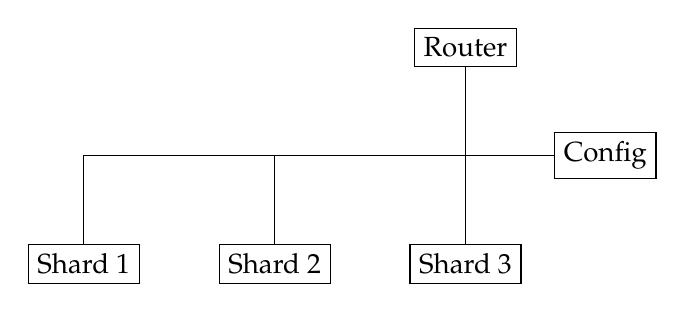
\begin{tikzpicture}
					
				\tikzstyle{block} = [rectangle,draw=black]
				
				\node[block] (r) {Router};
				\node[below=of r] (aux) {};
				\node[block,right=of aux] (c) {Config};
				\node[block,below=of aux] (s1) {Shard 3};
				\node[block,left=of s1] (s2) {Shard 2};
				\node[block,left=of s2] (s3) {Shard 1};
				
				\draw (r)--(s1);
				\draw (s2)|-(c);
				\draw (s3)|-(aux);
				\draw (c)--(aux);
				
			\end{tikzpicture}
			\caption{Arquitectura de datos de alta disponibilidad.}
			\label{fig:mongodb}
		\end{figure}
	
	\subsection{Capa de aplicación}
	\label{artAplicacion}
	
		Existen soluciones en la nube como por ejemplo \emph{Amazon Web Service (aws)}, \emph{Google Cloud} o \emph{Azure} que permiten crear rápidamente las aplicaciones. También es posible utilizar un sistema de orquestación escalable como \emph{kubernetes}.
	
	\subsection{Capa de negocio}
	\label{artNegocio}	
	
		Los sistemas en la nube también ofrecen facilidades para implementar una para de negocios. Existen además soluciones de código abierto que permiten construirla, como por ejemplo \emph{Grafana} o \emph{Checkmk}.

\section{Objetivos y alcance}
\label{objetivos}

%\chapter{Introducción Específica}
\label{Chapter2}

Este capítulo expone en detalle las tecnologías de todos los servicios que forman parte de la solución. Como así también el sistema de orquestación utilizado para que todas los componentes funcionen como una sola entidad.

	% Descripción de las plataformas tecnológicas que sostienen al trabajo
	\section{Tecnologías utilizadas}
	
	% Descripción de las dependencias del trabajo
	\section{Bibliotecas y paquetes de terceros}
	
	% Descripción de la planificación de las tareas, identificación y mitigación de riesgos.
	\section{Planificación} 
%\chapter{Diseño e Implementación}
\label{Chapter3}

	% Explicación sobre el funcionamiento y la creación de la arquitectura y del código que automáticamente despliega la aplicación en un servidor
	\section{Arquitectura y orquestación}

	% Explicación sobre el funcionamiento y la creación de los servicios que interactuan con dispositivos
	\section{Servicios orientados a dispositivos}
	
	% Explicación sobre el funcionamiento y la creación de los servicios que interactuan con el usuario
	\section{Servicios orientados a usuarios}
%\chapter{Ensayos y Resultados}
\label{Chapter4}

Párrafo introductorio del capítulo.

% Explicación de como se implementó TDD en algunos servicios y como se hicieron pruebas unitarias en otras
\section{Pruebas unitarias}

% Explicación del proceso de decición para determinar cuando debí realizar simulaciones. Descripción de las simulaciones creadas y su valides
\section{Simulaciones}

% Explicación del proceso de decición para determinar cuando debí realizar scripts. Descripción de las scripts creados y su valides
\section{Guiones y comandos}

% Recepción del cliente, sus comentarios y modificaciones realizadas para satisfacerlo
\section{Pruebas del cliente} 
%\chapter{Conclusiones}
\label{Chapter5}

Párrafo introductorio del capítulo.

% Valor agregado al cliente y mi aprendizaje
\section{Resultados obtenidos}

% Siguientes pasos para implementar el trabajo dentro del ambiente productivo de Gador
\section{Trabajo futuro} 

%-------------------------------------------------------------------------------
%	CONTENIDO DE LA MEMORIA  - APÉNDICES
%-------------------------------------------------------------------------------

\appendix

%\chapter{Appendix Title Here}
\label{AppendixA}

%\include{Appendices/AppendixB}
%\include{Appendices/AppendixC}

%-------------------------------------------------------------------------------
%	BIBLIOGRAPHY
%-------------------------------------------------------------------------------

\Urlmuskip=0mu plus 1mu\relax
\raggedright
\printbibliography[heading=bibintoc]

%-------------------------------------------------------------------------------

\end{document}  
